%!TEX program = pdflatex

\documentclass[a4paper, 12pt]{article}

\usepackage{geometry}
\geometry{a4paper,
total={170mm,257mm},left=2cm,right=2cm,
top=1cm,bottom=2cm}

\usepackage{mathtext}
\usepackage{amsmath}
\usepackage[T2A]{fontenc}
\usepackage[utf8]{inputenc}
\usepackage[english,russian]{babel}
\usepackage{graphicx, float}
\usepackage{tabularx, colortbl}
\usepackage{caption}
\captionsetup{labelsep=period}

\newcommand{\parag}[1]{\paragraph*{#1:}}
\DeclareSymbolFont{T2Aletters}{T2A}{cmr}{m}{it}
\newcounter{Points}
\setcounter{Points}{1}
\newcommand{\point}{\arabic{Points}. \addtocounter{Points}{1}}
\newcolumntype{C}{>{\centering\arraybackslash}X}

\begin{document}
%\maketitle

\begin{titlepage}
    \vspace*{\fill}
    
    \begin{center}
        
\includegraphics[scale=0.8]{res/MIPT.pdf}
        \\[0.7cm]\Huge Московский Физико-Технический Институт
        \\[2cm]\LARGE Отчет о выполнении лабораторной работы 
        \\[0.5cm]\noindent\rule{\textwidth}{1pt}
        \\\Huge\textbf{5.5.2 \\ Спектрометрия $\alpha$-излучения с помощью полупроводникового детектора}
        \\[-0.5cm]\noindent\rule{\textwidth}{1pt}
    \end{center}
    
    \vspace*{\fill}
    
    \begin{flushleft}
        Выполнили: \hspace{\fill} Группа:
        \\Костылев Владислав и Шишакова Ксения\hspace{\fill} Б01-206
    \end{flushleft}
\end{titlepage}

\setcounter{page}{2}


\begin{abstract}
    \textbf{Цель работы:} C помощью кремниевого поверхностно-барьерного детектора измеряются спектры $\alpha$-частиц, испускаемых различными радиоактивными ядрами - ${ }^{226} \mathrm{Ra},{ }^{238} \mathrm{U},{ }^{241} \mathrm{Am} + ^{230} \mathrm{Th}$ и ${ }^{239} \mathrm{Pu}$. Исследуется тонкая структура $\alpha-$ излучения и последовательность радиоактивных распадов в семействе урана.
\end{abstract}

\tableofcontents
\newpage

\section{Теоретическая справка} 

    К числу радиоактивных процессов относятся $\alpha$- и $\beta$-распады (в том числе и $K$-захват), $\gamma$-излучение, деление ядер, а также испускание запаздывающих нейтронов и протонов. В этой работе изучается $\alpha$-распад.\\
    Энергию вылетающих из ядра $\alpha$-частиц легко подсчитать на основе законов сохранения. Если родительское (исходное) ядро имеет массу $M_1$, а дочернее (конечное) - $M_2$, то законы сохранения энергии и импульса записываются в форме

    $$
    \begin{gathered}
    M_2 c^2=M_1 c^2+m_\alpha c^2+T_1+T_\alpha, \\
    \mathrm{p}_1+\mathrm{p}_\alpha=0
    \end{gathered}
    $$

    где $T_1$ и $\mathrm{p}_1$ - кинетическая энергия и импульс отдачи дочернего ядра, a $T_\alpha$ и $\mathrm{p}_\alpha$ - кинетическая энергия и импульс $\alpha$-частицы.

    Ясно, что вылет $\alpha$-частицы из ядра возможен лишь в том случае, если разность энергий покоя родительского и дочернего ядра будет больше энергии покоя $\alpha$-частицы. В силу того, что реально $\alpha$-распад испытывают лишь тяжелые ядра с $A>200$, энергия отдачи ядра очень мала и фактически кинетическая энергия $\alpha$-частицы равна разности энергий покоя исходного и конечного ядер. Именно поэтому вылетающие $\alpha$-частицы имеют строго определенную энергию.

    Однако экспериментально обнаружено, что энергетический спектр $\alpha$-частиц многих $\alpha$-активных ядер состоит из нескольких линий, одна из которых преобладающее. Дискретность линий и их относительная интенсивность объяснимы, поскольку, во-первых, $\alpha$-частицы могут испускаться ядром, находящимися в возбужденном состоянии (длиннопробежные $\alpha$-частицы), а во-вторых может происходить $\alpha$-распад из основного состояния родительского ядра на возбужденные состояния дочернего ядра (короткопробежные $\alpha$-частицы). Так как период полураспада для $\alpha$-частиц примерно в $10^5$ раз больше периода $\alpha$-распада, то интенсивность длиннопробежных $\alpha$-частиц очень мала.

    Тяжелые ядра, как правило, в основном состоянии деформированы (исключением являются магические ядра). Это означает, что низколежащими состояниями являются вращательные полосы, и именно на эти состояния обычно и происходит распад родительского ядра, приводящий к появлению группы короткопробежных $\alpha$-частиц. Как известно, энергия вращательных уровней определяется выражением

    $$
    E_\text{вp}=\frac{\hbar^2}{2 \mathcal{I}} l(l+1).
    $$

    Тем самым измерение тонкой структуры энергетического спектра $\alpha$ частиц дает возможность определить момент инерции ядра $\mathcal{I}$.

    Периоды полураспада $\alpha$-активных ядер очень сильно зависят от энергии вылетающих частиц. Экспериментально установленная зависимость (закон Гейгера-Нэттола) имеет вид:

    \begin{equation}\label{eq:gey_net}
    \lg T_{1 / 2}=\frac{a}{\sqrt{E_\alpha}}+b .
    \end{equation}

    Коэффициенты $a$ и $b$ очень слабо зависят от заряда ядра $Z$.


\section {Экспериментальная установка}

    В состав экспериментальной установки входят альфа-спектрометр, форвакуумный насос и персональный компьютер:

    \begin{figure}[H]
        \centering
        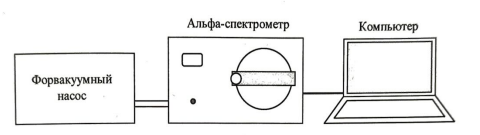
\includegraphics[width=0.7\linewidth]{res/1.png}
    \end{figure}

    Форвакуумный насос, соединенный с корпусом альфа-спектрометра вакуум-ным шлангом, откачивает измерительную камеру до давления 0,2 мм рт. ст.\\
    Установка автоматически поддерживает давление в измерительной камере в рабочем диапазоне от 0,2 до 2,0 мм рт. ст. Откачка блокируется при разгерметизации камеры. Соединение и отсоединение измерительной камеры с атмосферой осуществляется с помощью двух электромагнитных клапанов.\\
    Внешний вид альфа-спектромерта изображен рисунке ниже:

    \begin{figure}[H]
        \centering
        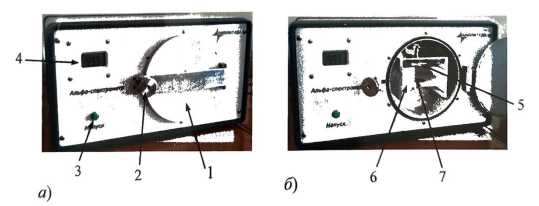
\includegraphics[width=0.7\linewidth]{res/2.png}
    \end{figure}

    Здесь 1 - крышка измерительной камеры, 2 - прижимная ручка, 3 - кнопка разгерметизации (напуска атмосферы), 4 - индикатор давления в камере (показывает давление в мм рт. ст.). Внутри измерительной камеры альфа-спектрометра (рис. 26) располагается полупроводниковый детектор 5, держатель образца 6 вместе с металлической подложкой 7, на которую устанавливают образцы с радиоактивными источниками. Металлическая подложка 7 соединена гибким проводником с источником постоянного напряжения. На подложку 7 подается отрицательный потенциал (относительно корпуса измерительной камеры) для того, чтобы ядра отдачи, получившие импульс, направленный вверх, не попадали на детектор и не загрязняли его. Держатель образца 6 вместе с самим образцом можно располагать на нескольких фиксированных расстояниях от детектора. Электрический сигнал с полупроводникового детектора усиливается, поступает на плату аналогово-цифрового преобразователя (АЦП) и обрабатывается компьютером.

    Амплитуда электрического сигнала с полупроводникового детектора пропорциональна энергии а - частицы, и поэтому с помощью компьютера мы регистрируем спектры источников. Осуществляется это с помощью установленной на компьютере программы "Прогресс"

    При использовании детектора в спектрометрических целях особое значение приобретает его разрешающая способность, т. е. ширина кривой распределения импульсов по амплитудам при строго постоянной энергии регистрируемых частиц. Форма такой кривой распределения обычно бывает близка к кривой ошибок (гауссовой кривой)

    $$
    W(U) d U=\frac{1}{\sqrt{2 \pi} \sigma} e^{-\left(U-U_0\right)^2 /\left(2 \sigma^2\right)} d U
    $$

    Распределение (5) имеет вид колокола с максимумом при $U=U_0$. Разрешающую способность спектрометра определяют по величине $\delta$ ширине кривой $W(U)$, измеренной на половине высоты. Энергетическим разрешением спектрометра обычно называют величину

    $$
    R=\frac{\delta}{U_0} \cdot 100 \% .
    $$

    Нетрудно найти связь между $\delta$ и б:

    $$
    \delta=2 \sqrt{2 \ln 2} \sigma .
    $$

    Одной из основных причин, вызывающих разброс импульсов по амплитуде, является статистическая флуктуация числа электрондырочных пар, создаваемых падающей частицей. Среднее число пар $N$ равно

    $$
    N=E / E_{\mathrm{cp}},
    $$

    где $E$ - энергия, теряемая частицей в детекторе, а $E_{\mathrm{cp}}=3.6$ эВ - энергия, необходимая для создания пары электрон-дырка. Среднеквадратичное отклонение $\sigma$ равно

    $$
    \sigma=\sqrt{N}=\sqrt{E / E_{\mathrm{cp}}}
    $$

    Вклад флуктуаций числа пар в энергетическое разрешение

    $$
    R_{\text {флук }}=\frac{\sigma}{N} \cdot 100 \%=\sqrt{\frac{E_{\mathrm{cp}}}{E}} \cdot 100 \% .
    $$
    
    
\section{Результаты измерений и обработка данных} 

    Сперва по спектру откалибруем номера каналов в энергетических единицах (МэВ). Будем использовать спектр ${ }^{226} \mathrm{Ra}$ для калибровки.

    Номера пиков: $N_1 = 1677, N_2 = 1930, N_3 = 2100, N_4 = 2690$. Им соответствуют табличные значения: $4.784, 5.490, 6.002, 7.687$ МэВ.

    $$ a = (2.87 \pm 0.02) \cdot 10^{-3} \; \frac{ \text{МэВ} }{ \text{кан.} }$$
    $$ b = (-0.04 \pm 0.04) \; \text{МэВ}$$

    \begin{figure}[H]
        \centering
        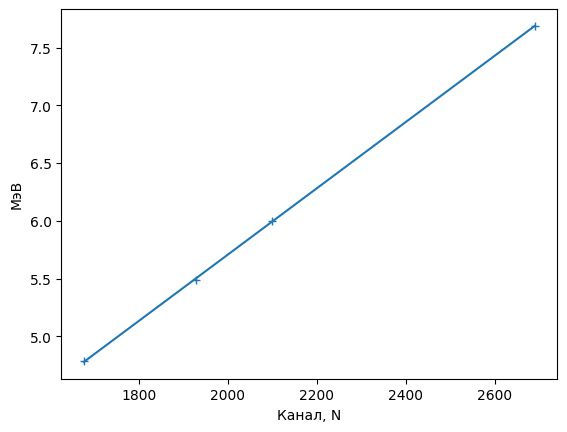
\includegraphics[width=0.7\linewidth]{res/3.png}
    \end{figure}

    для ${ }^{226} \mathrm{Ra}$
    \begin{figure}[H]
        \centering
        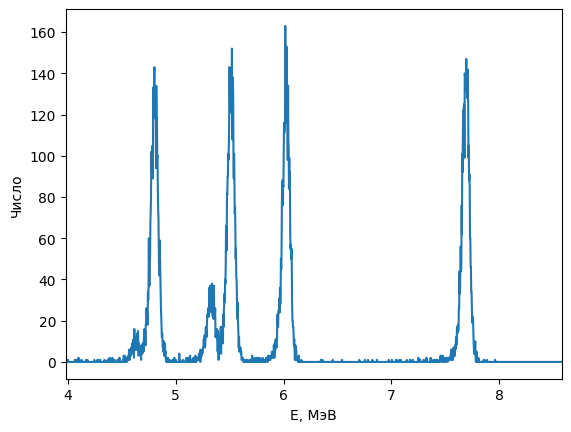
\includegraphics[width=0.6\linewidth]{res/4.png}
    \end{figure}

    Для ${ }^{239} \mathrm{Pu}$
    \begin{figure}[H]
        \centering
        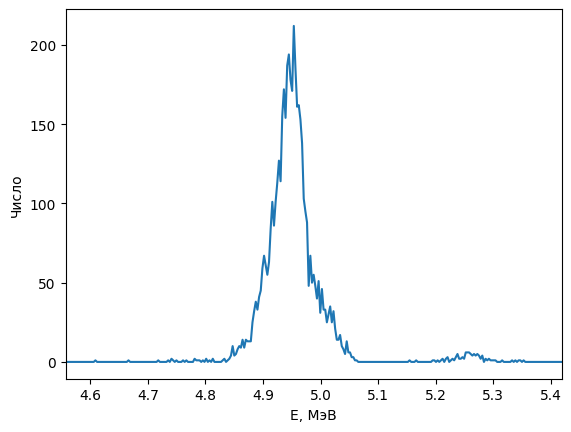
\includegraphics[width=0.6\linewidth]{res/6.png}
    \end{figure}
    
    Для ${ }^{241} \mathrm{Am} + { }^{230} \mathrm{Th}$
    \begin{figure}[H]
        \centering
        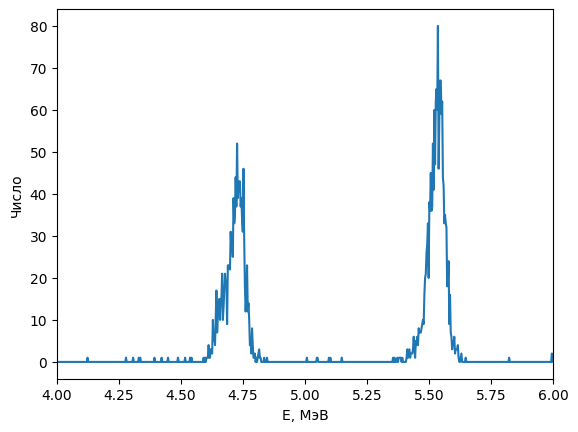
\includegraphics[width=0.6\linewidth]{res/7.png}
    \end{figure}

    Для ${ }^{238} \mathrm{U}$
    \begin{figure}[H]
        \centering
        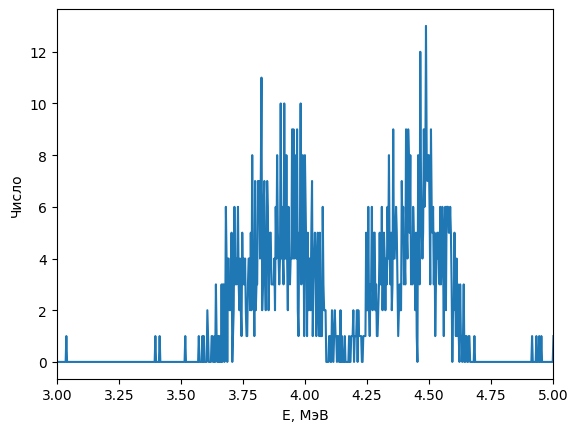
\includegraphics[width=0.6\linewidth]{res/8.png}
    \end{figure}

    \begin{figure}[H]
        \centering
        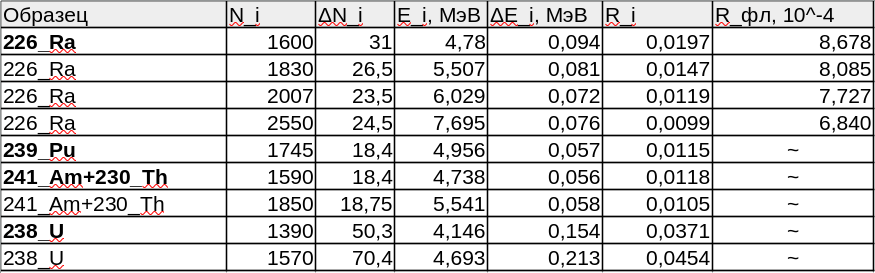
\includegraphics[width=0.7\linewidth]{res/5.png}
    \end{figure}

    Проверим закона Гейгера-Нетолла:
    \begin{figure}[H]
        \centering
        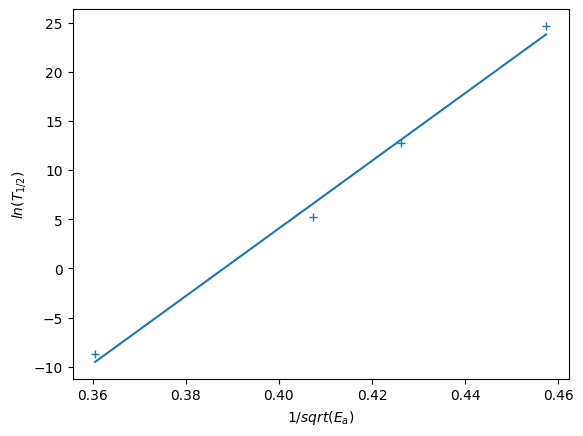
\includegraphics[width=0.7\linewidth]{res/9.png}
    \end{figure}

    
\section{Заключение}
    В заключение, хочу отметить, что с помощью кремниевого поверхностно-барьерного детектора мы измерили спектры $\alpha$-частиц, испускаемых различными радиоактивными ядрами - ${ }^{226} \mathrm{Ra},{ }^{238} \mathrm{U},{ }^{241} \mathrm{Am} + ^{230} \mathrm{Th}$ и ${ }^{239} \mathrm{Pu}$. 
    А также исследовали тонкую структуру $\alpha-$ излучения и последовательность радиоактивных распадов в семействе урана.
    
\end{document}
